%!TEX root = /Users/simo/Documents/PFC/memoria/memoria.tex
\section{Segundo Ciclo} % (fold)
\label{sec:secundo_ciclo}

Se considera interesante que la siguiente evolución de la aplicación sea la introducción del concepto de Usuario.

\subsection{Análisis de requisitos} % (fold)
\label{sub:análisis_de_requisitos}

\begin{itemize}
  \item Poder registrarse en la web de la forma más simple posible.
  \item Tener un panel sencillo desde el que manejar sus documentos
  \item Seguridad básica para que no se pueda acceder a elementos que no se debería tener acceso.
\end{itemize}

% subsection análisis_de_requisitos (end)

\subsection{Diseño} % (fold)
\label{sub:diseño}

En cuanto al diagrama de clases del dominio, en este caso aparece un nuevo modelo usuario \texttt{User}, el cual tiene varios \texttt{Document}'s, y tiene los atributos básicos de nombre de usuario (\texttt{login}), \texttt{email} y \texttt{password}.

\begin{figure}[h!]
\centering
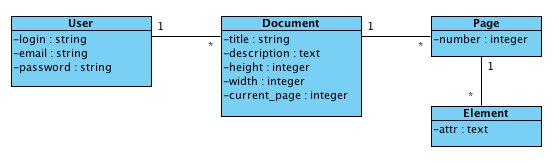
\includegraphics[width=15cm]{uml2.png}
\caption{Clases del dominio, 2º ciclo}\label{fig:uml2}
\end{figure}

Para manejar todo el proceso de registro, y cualquiera del resto de acciones necesarias, si llegara el caso de recuperar contraseña, dar de baja, o editar los datos de usuario, se cree necesario crear otro controlador diferente, al que se llamará \texttt{users\_controller}. También, al tener en este caso una parte privada y una parte pública de la web, es necesario tener una serie de acciones que no tienen que ver ni con manejar documentos ni con registrarse. Por ello, y para cualquier otra acción sencilla que se quiera añadir en un futuro referente a lo que sería la web en si (página de contacto, ayuda, información del autor, etc), se ha decidido crear un controlador extra llamado \texttt{website\_controller}.

% subsection diseño (end)

\subsection{Implementación} % (fold)
\label{sub:implementación}

\subsubsection{Registro de usuarios} % (fold)
\label{ssub:registro_de_usuarios}

El proceso de manejo de usuarios es un tema muy delicado en cuanto a seguridad se refiere. Existen sobradas razones para blindar totalmente este proceso, que la contraseña esté guardada de forma encriptada, y que los datos que introduce el usuario estén seguros. Y puesto que la funcionalidad de poder registrarse en una web es algo tan común en el mundo de las webs, existe alguien que se ha encargado de facilitar todo este proceso en forma de plugin para Rails.

Los plugins pueden servir para multitud de propósitos, y suelen solucionar necesidades comunes de las webs que Rails no incluye para no sobrecargar el Framework. En este caso el plugin se llama \texttt{restful\_authentication} \footnote{\url{http://github.com/technoweenie/restful-authentication}}. Este plugin se encarga de las tareas de registro de usuarios creando un modelo llamado User, tal y como se había planeado, y un controlador con las funciones de registro (\texttt{signup}), login y logout. Además, aporta una serie de funciones de ayuda (\texttt{helpers} en Rails), que permiten tratar en todo momento con el usuario, y por ejemplo, saber si la persona que está realizando una petición de una página está logueado o no. 

Este plugin utiliza la técnica de salted passwords \footnote{\url{http://en.wikipedia.org/wiki/Salt\_(cryptography)}} para almacenar las contraseñas en la base de datos. Ésta técnica genera una cadena aleatoria (salt) de 40 caracteres mediante \texttt{SHA1}, que se utiliza para generar el llamado salted password, también de 40 caracteres mediante \texttt{SHA1}. Se considera el standard de facto en cuanto a registro y guardado de contraseñas se refiere, y es una técnica utilizada en numerosos protocolos criptográficos, como por ejemplo SSL. Esta encriptación dificulta los ataques a contraseñas mediante diccionario de forma exponencial, puesto que por cada palabra \emph{común} de los diccionarios usados, es necesario tener las $2^{160}$ posibles combinaciones introducidas por el salt de 160 bits. Incluso si la base de datos se comprometiera, y un atacante tuviera acceso a alguno de los campos, tanto el salt, como el password encriptado, aún debería romper la clave mediante el método tradicional, puesto que ya sabría cual es el salt, pero seguiría teniendo que encontrar cual es la clave que, añadida al salt, y encriptándola mediante SHA1, genera el password encriptado.

Este plugin requiere de el campo extra salt, que no se había planteado en un principio en la etapa de diseño.

% subsubsection registro_de_usuarios (end)

\subsubsection{Panel de control} % (fold)
\label{ssub:panel_de_control}

Mediante el plugin de usuarios es cuestión de controlar si se está logueado o no para mostrar la pantalla inicial de la web, del controlador \texttt{website\_controller}, o la pantalla con el \emph{panel de control} del usuario, también dentro del mismo controlador. El siguiente paso es evolucionar el Scaffold de documentos para controlar que en todo momento, solo el propietario de los documentos pueda realizar las acciones solicitadas.

Así, por ejemplo, las funciones del \texttt{documents\_controller} evolucionan de unas líneas como las siguientes:

\begin{verbatim}
  def update
    @doc = Document.find(params[:id])
    @doc.update_attributes params[:document]
    redirect_to :action => "edit", :id => @doc.id
  end
\end{verbatim}

A algo como lo siguiente:

\begin{verbatim}
  def update
    @doc = Document.find(params[:id])
    redirect_to :action => :index unless @doc.user == current_user
    @doc.update_attributes params[:document]
    redirect_to :action => "edit", :id => @doc.id
  end
\end{verbatim}

Dichos cambios son mínimos, por la simplicidad en que todos ellos están implementados. La parte de comunicación con Javascript, de momento, se dejará abierta hasta que se decida qué política se aplicará para permitir o no a los usuarios ver o editar sus contenidos.

% subsubsection panel_de_control (end)

% subsection implementación (end)

% section secundo_ciclo (end)